\newcommand{\code}[1]{\colorbox{lightgray}{\texttt{#1}}}

\section{Simulation Code}
\label{sim}

First, the logic of the game was coded in Python. A \code{Player} class was created to make it convenient to hold and handle transactions of coins between the players and the pot, and the two players and the pot were created as \code{Player} objects. A \code{for} loop was created, which would run iterations as specified by \code{num\_trials}. A nested \code{while} loop was created, which would run until a player had to put their coins into the pot but had none left. The number of cycles until the end of the game was recorded in a list, and the process was repeated. At the end of \code{num\_trials} iterations, the code plotted a histogram showing the distribution of the number of cycles, and calculated the mean of the distribution of cycles.

Some quality-of-life improvements were also made, such as using the \code{tqdm} package to show a progress bar as the code was performing iterations, and using \code{bashplotlib} to plot an ASCII version of the histogram in the command-line as the code was executing, an example of which can be seen in Figure \ref{fig:bashplot}. This code can be seen in the project's GitHub repository\footnote{\texttt{https://github.com/kadhirumasankar/isye-6739-project}}, as well as in Appendix \ref{pythoncode}.

\begin{figure}[H]
\centering
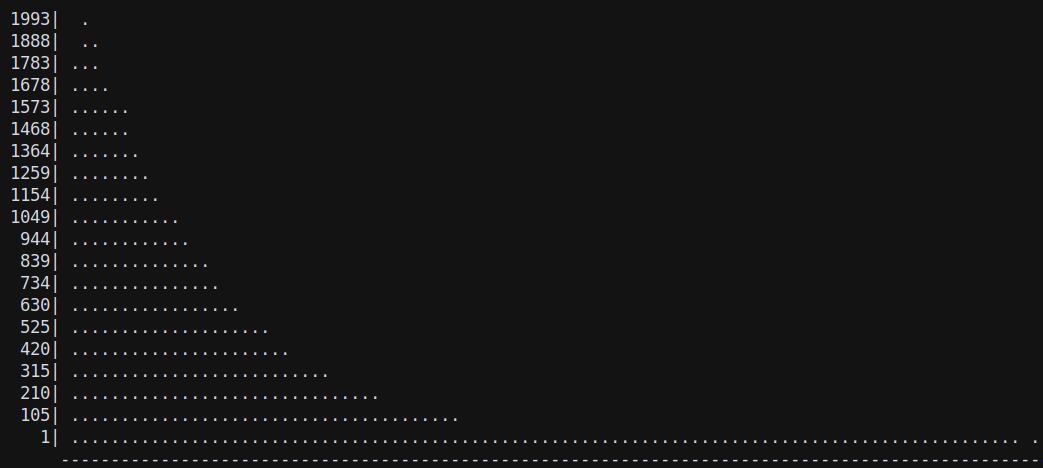
\includegraphics[width=.75\textwidth]{bashplot.png}
\caption{Screenshot of a histogram on the command-line, plotted using \code{bashplotlib}, to allow users to see changes in the distribution as the code is executing}
\label{fig:bashplot}
\end{figure}